%%%%%%%%%%%%%%%%%%%%%%%%%%%%%%%%%%%%%%%%%%  不使用 authblk 包制作标题  %%%%%%%%%%%%%%%%%%%%%%%%%%%%%%%%%%%%%%%%%%%%%%
%-------------------------------PPT Title-------------------------------------
\title{24-选讲专题:~机器学习方法简介}
%-----------------------------------------------------------------------------
%----------------------------Author & Date------------------------------------

%\author[\textrm{Jun\_Jiang}]{姜\;\;骏\inst{}} %[]{} (optional, use only with lots of authors)
%% - Give the names in the same order as the appear in the paper.
%% - Use the \inst{?} command only if the authors have different
%%   affiliation.
%\institute[BCC]{\inst{}%
\institute[Gain~Strong]{\inst{}%
%\vskip -20pt 北京市计算中心}
\vskip -20pt {\large 格致斯创~科技}}
\date[\today] % (optional, should be abbreviation of conference name)
{%	{\fontsize{6.2pt}{4.2pt}\selectfont{\textcolor{blue}{E-mail:~}\url{jiangjun@bcc.ac.cn}}}
\vskip 45 pt {\fontsize{8.2pt}{6.2pt}\selectfont{%清华大学\;\;物理系% 报告地点
	\vskip 5 pt \textrm{2023.04.22}}}
}

%% - Either use conference name or its abbreviation
%% - Not really information to the audience, more for people (including
%%   yourself) who are reading the slides onlin%%   yourself) who are reading the slides onlin%%   yourself) who are reading the slides onlineee
%%%%%%%%%%%%%%%%%%%%%%%%%%%%%%%%%%%%%%%%%%%%%%%%%%%%%%%%%%%%%%%%%%%%%%%%%%%%%%%%%%%%%%%%%%%%%%%%%%%%%%%%%%%%%%%%%%%%%

\subject{}
% This is only inserted into the PDF information catalog. Can be left
% out.
%\maketitle
\frame
{
%	\frametitle{\fontsize{9.5pt}{5.2pt}\selectfont{\textcolor{orange}{“高通量并发式材料计算算法与软件”年度检查}}}
\titlepage
}
%-----------------------------------------------------------------------------

%------------------------------------------------------------------------------列出全文 outline ---------------------------------------------------------------------------------
%\section*{}
%\frame[allowframebreaks]
%{
%  \frametitle{Outline}
%%  \frametitle{\textcolor{mycolor}{\secname}}
%  \tableofcontents%[current,currentsection,currentsubsection]
%}
%%在每个section之前列出全部Outline
%%类似的在每个subsection之前列出全部Outline是\AtBeginSubsection[]
%\AtBeginSection[]
%{
%  \frame<handout:0>%[allowframebreaks]
%  {
%    \frametitle{Outline}
%%全部Outline中,本部分加亮
%    \tableofcontents[current,currentsection]
%  }
%}

%-----------------------------------------------PPT main Body------------------------------------------------------------------------------------
\small
%\section{\rm{VASP~}软件中\rm{PAW~}计算的实现}
%\frame
%
%	\frametitle{\textrm{VASP}计算的特色}
%	相比于与普通的第一原理计算软件,\textrm{VASP}很好地平衡了计算效率和精度的问题,总的来说,\textrm{VASP}主要通过这几个特色保证了计算的高效能
%	\begin{itemize}
%	     \item 迭代与优化算法的多样性\\
%		     本质上电荷密度迭代 \textrm{\&\&} 体系总能量优化是相同的优化问题,采用了类似的算法\upcite{CMS6-15_1996,PRB54-11169_1996}:\\
%			\textcolor{blue}{\textrm{Pseudo-Newton、Conjugate-Gradient、Broyden~mix、damping-factor、RMM-DIIS}}
%	     \item 尽可能采用局域基(原子轨道基)函数:~\\
%		     \textcolor{blue}{\textrm{LREAL}}=\textcolor{red}{\textrm{.TRUE.}}\\
%			优化的投影函数也尽可能在实空间表示
%	     \item \textrm{PAW}原子数据集:\textcolor{blue}{优异的赝势}\upcite{PRB59-1758_1999}
%	\end{itemize}
%}
\frame
{
	\frametitle{科学研究的范式变更}
\begin{figure}[h!]
\vspace*{0.08in}
\centering
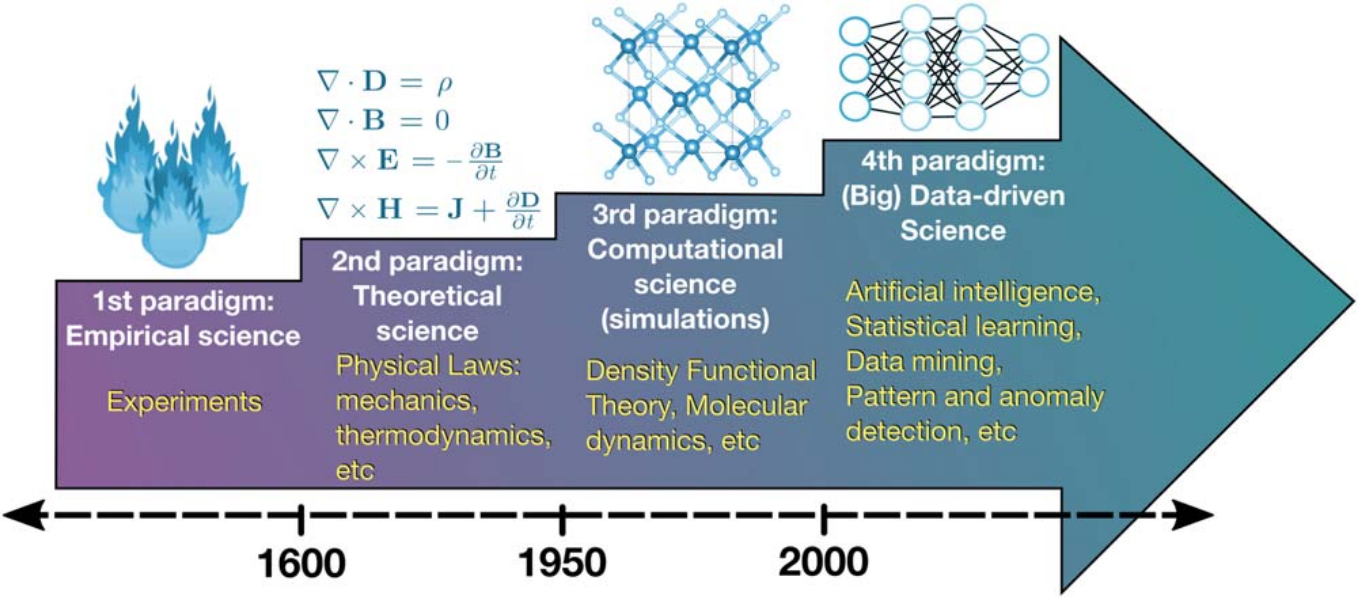
\includegraphics[height=2.00in,width=4.15in]{Figures/Four_Model_3.png}
%\caption{\tiny \textrm{Pseudopotential for metallic sodium, based on the empty core model and screened by the Thomas-Fermi dielectric function.}}%(与文献\cite{EPJB33-47_2003}图1对比)
\label{Four_Model}
\end{figure}
}

\section{机器学习简介}
\frame
{
	\frametitle{机器学习\textrm{(Machine Learning, ML)}}
机器学习是自动完成数据分析并提取数据关系的一类方法的统称
\begin{figure}[h!]
\centering
\vspace*{-0.1in}
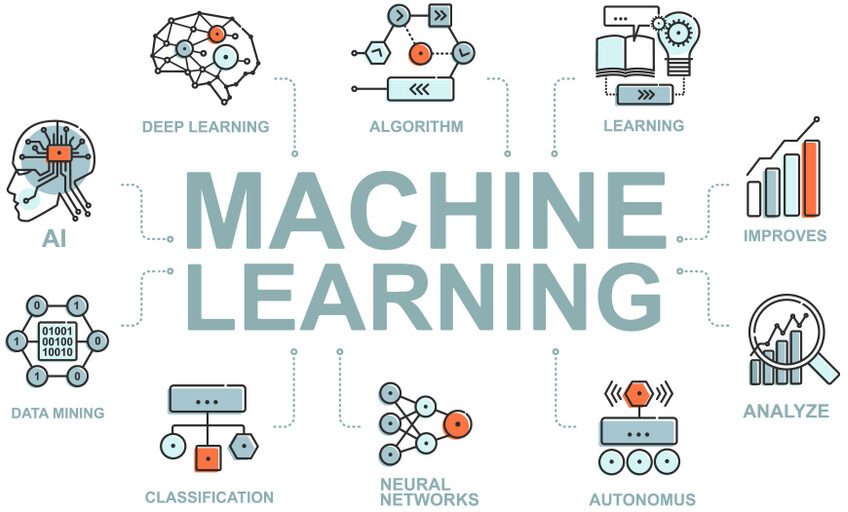
\includegraphics[height=2.3in,width=3.8in,viewport=0 0 630 390,clip]{Figures/Machine_Learning.jpg}
%\caption{\fontsize{7.2pt}{4.2pt}\selectfont{\textrm{人工智能与机器学习和深度学习的层次关系示意图.引自文献\cite{JPM2-032001_2019}}}}%
\label{Machine-Learning}
\end{figure}
\textcolor{blue}{用已知的数据关系预测未知数据或辅助不确定条件下的决策过程}
}

\frame
{
	\frametitle{人工智能\textrm{(Artificial Intelligence, AI)}与机器学习}
		获取材料完整物性数据的成本,无论是通过实验手段还是计算模拟,代价都是比较高
		\begin{itemize}
			\item 高通量第一原理计算自动流程和数据库解决了材料物性数据的获取问题%,但是并未给出现有材料数据基础上的物性优化的方案
			\item 利用数据挖掘技术,实现数据驱动的材料物性筛选、预测和提升的技术路线,有着特殊重要的意义
		\end{itemize}
	\vskip 8pt
	{\fontsize{8.2pt}{6.2pt}\selectfont{任何计算机模拟人类智能的算法都可以划归为人工智能,并非一定要应用机器学习算法,也包括决策树、知识库、计算机逻辑等算法
		\vskip 3pt
		{\fontsize{6.8pt}{4.2pt}\selectfont{\textcolor{blue}{人工智能广泛应用于金融、导航控制、语言处理、游戏竞技、计算机可视化和生物信息学等领域}}}
	\begin{itemize}
		\item 机器学习技术可以从大量数据中获得有价值的信息,尤其是面对高维复杂数据时,机器学习技术是确定数据间关系的有力的工具
	\item 机器学习领域的深度学习\textrm{(Deep Learning, DL)}是仿照生物神经网络\footnote{\fontsize{7.2pt}{6.2pt}\selectfont{神经网络结构意味着输入输出之间允许有多个类似神经的网络层}}结构为主要代表的一种示类学习
\end{itemize}}}
}

\frame
{
	\frametitle{人工智能和机器学习的层次关系}
	传统定义界定的机器学习,是指无须借助解析程序,直接依靠数据来提升任务处理的性能,自从\textrm{1950}年代统计学、计算科学与技术和神经科学的发展,机器学习的研究发展到了更广泛的人工智能领域%图\ref{AI-ML}表明了人工智能和机器学习的层次关系。
\begin{figure}[h!]
\centering
\vspace*{-0.1in}
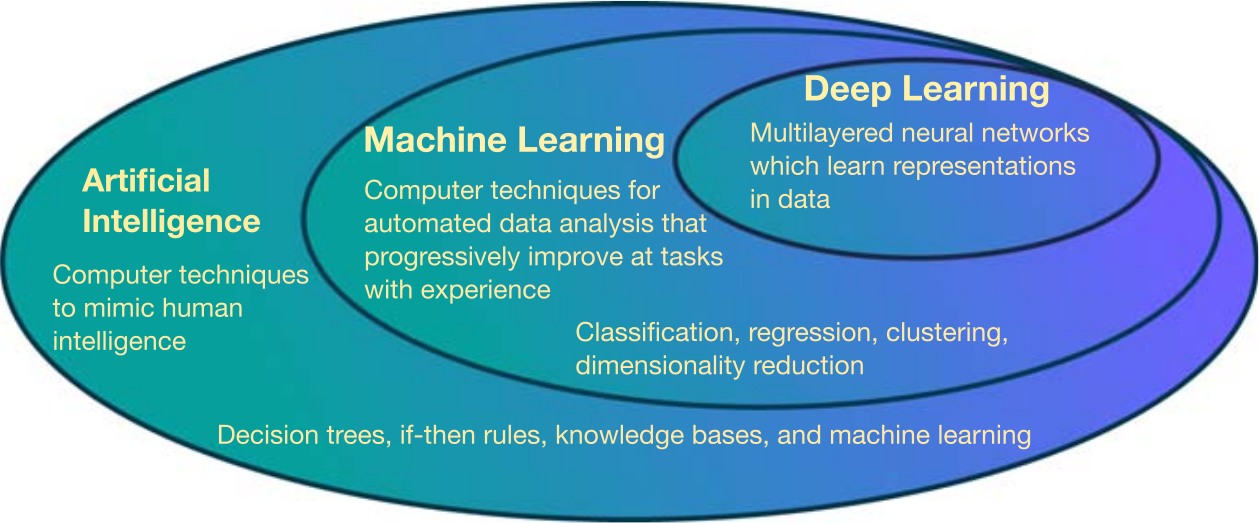
\includegraphics[height=1.9in,width=4.0in,viewport=0 0 1275 550,clip]{Figures/Hierarchical_description_AI_ML_DL.png}
\caption{\tiny{\textrm{Artificial Intelligence, Machine Learning and Deep Learning.}}}%
\label{AI-ML}
\end{figure}
}

\frame
{
	\frametitle{机器学习问题的一般形式与分类}
	\begin{itemize}
		\item 机器学习类问题的一般表示:
\vskip 5pt
对于给定的集合$\mathbf{X}$,可以预测或近似得到未知函数$y=f(\mathbf{X})$
\vskip 4pt
{\fontsize{6.2pt}{4.2pt}\selectfont{
	集合$\mathbf{X}$构成特征空间,集合中的每个元素$\mathbf{x}$称为特征向量(在材料类的机器学习中也称描述符)\\
	根据机器学习得到的近似函数$\hat{y}=\hat{f}(\mathbf{X})$,模型有能力预测训练数据之外的输出值}}
\vskip 5pt
	\textcolor{blue}{\fontsize{8.0pt}{4.2pt}\selectfont{机器学习的这种预测能力也称为模型的“泛化”\textrm{(generalization)}}}
\item 机器学习主要根据学习的特征分为无监督学习\textrm{(unsupervised learning)}和监督学习\textrm{(supervised learning)}
	\item 此外的机器学习问题还包括:~
\begin{itemize}
	\item 半监督学习,即大部分没有映射关系的数据和少量有映射关系的数据;
	\item 多任务和迁移学习,即将从相关问题习得的知识应用到数据极少的对象,提升模型的学习能力
	\item 强化学习,即没有输入输出,但会和环境不断交互,通过最大化环境的反馈,最终达到学习目标
\end{itemize}
	\end{itemize}
}

\frame
{
	\frametitle{无监督学习}
无监督学习是描述性质的,所有数据只有特征向量,没有标签,但呈现出聚群的结构,相似类型或特征的数据会聚集在一起
\begin{itemize}
	\item 如果没有标签的数据的组合是有限个,称为聚类\textrm{(clustering)};~无限的称为密度估计\textrm{(density estimation)}
	\item 将高维数据投影到低维空间,称为降维\textrm{(dimensionality reduction)}
		\vskip 2pt
		{\fontsize{8.0pt}{4.2pt}\selectfont{降维有助于了解复杂数数据的检测模式}}
%	\item 识别数据中的异常点或离群点
%		\vskip 2pt
%		{\fontsize{8.0pt}{4.2pt}\selectfont{异常检测可用于欺诈检测、故障预警等场景}}
\end{itemize}
\begin{figure}[h!]
\centering
\vspace*{-0.1in}
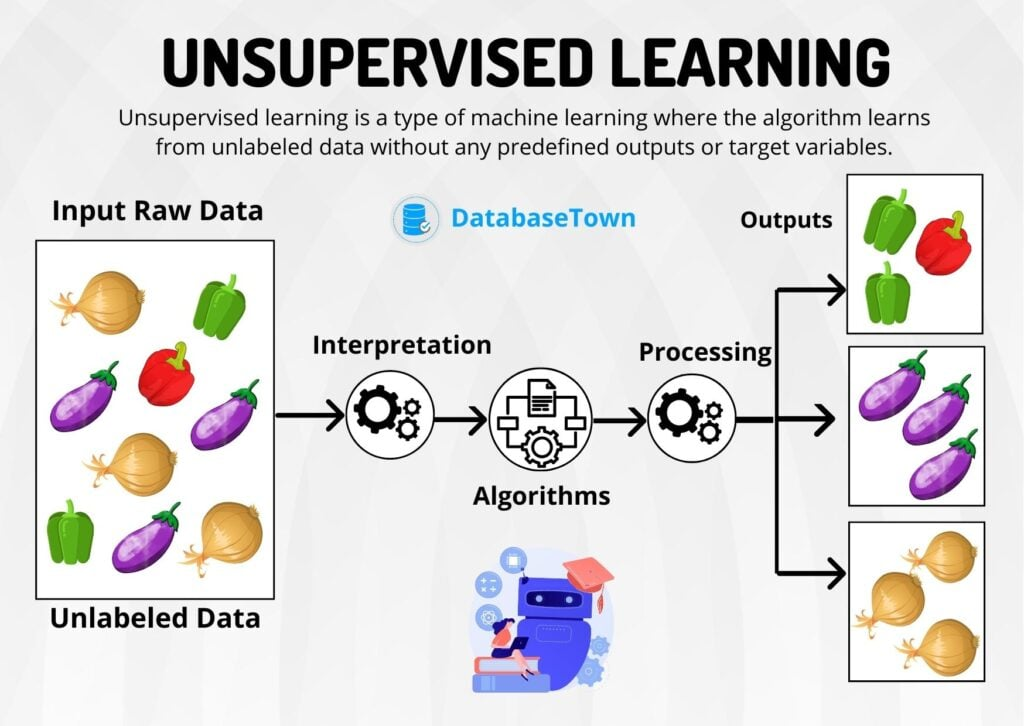
\includegraphics[height=1.5in,width=2.7in,viewport=0 0 1075 720,clip]{Figures/ML_Unsupervised-Learning.jpg}
\caption{\tiny{\textrm{The Schematic diagram of Unsupervised Learning.}}}%
\label{ML_Unsupervised-Learning}
\end{figure}
}

\frame
{
	\frametitle{监督学习}
	监督学习是通过学习指定数量的输入输出间的函数映射
\begin{itemize}
	\item 如果输出函数$y_{\mathrm{i}}$表示类别的有限集合,称为分类\textrm{(classification)}问题
		\vskip 2pt
		{\fontsize{8.0pt}{4.2pt}\selectfont{模型可用来预测未知数据所属类型}}
	\item 如果输出函数$y$是实数,称为回归\textrm{(regression)}问题
		\vskip 2pt
		{\fontsize{8.0pt}{4.2pt}\selectfont{模型可用来预测未知输入数据对应的值输出值}}
\end{itemize}
\begin{figure}[h!]
\centering
\vspace*{-0.1in}
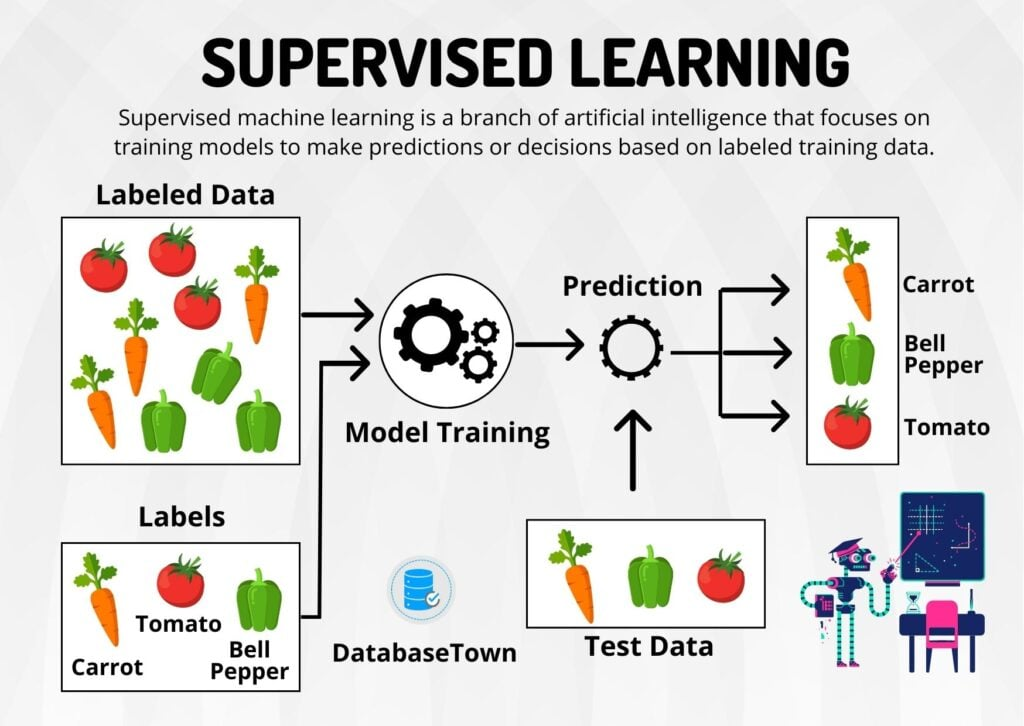
\includegraphics[height=1.6in,width=2.8in,viewport=0 0 1075 720,clip]{Figures/ML_Supervised-Learning-2.jpg}
\caption{\tiny\selectfont{\textrm{The Schematic diagram of Supervised Learning.}}}%
\label{ML_Supervised-Learning}
\end{figure}
}

\frame
{
	\frametitle{机器学习的流程}
\begin{itemize}
	\item \textcolor{blue}{数据的收集和筛选}:~{\fontsize{8.0pt}{4.2pt}\selectfont{从现有数据中产生并选择与问题解决有用和相关的数据子集}}
	\item \textcolor{blue}{数据预处理}:~清洗缺失和不完整数据,将数据将转换成统一的格式{\fontsize{8.0pt}{4.2pt}\selectfont{(如整型、字符串型等)}}%。必要时还须根据需要将数据按问题的格式重新表示
	\item \textcolor{blue}{数据训练}:~将数据分为训练集、验证集和测试集三部分,训练集数据用于学习并得到模拟参数{\fontsize{8.0pt}{4.2pt}\selectfont{(主要针对监督学习)}}
	\item \textcolor{blue}{模型测试和优化}:~用验证集数据评估模型的效果和性能,并用验证集数据优化模型
		\vskip 3pt
		{\fontsize{8.0pt}{4.2pt}\selectfont{一旦完成优化,用测试集数据评定模型的性能}}%。如果学习不成功,选用改善的数据重复上述步骤或改变学习算法。
	\item \textcolor{blue}{模型应用}:~将得到的有效模型对未知数据进行预测,如果有新的数据,模型还可以继续训练
\end{itemize}
}

\section{机器学习算法}
\frame
{
	\frametitle{主成分分析}
	主成分分析\textrm{(principal component analysis, PCA)}:\\
	{\fontsize{8.0pt}{4.2pt}\selectfont{\textcolor{blue}{将高维数据投影到数据点集中的区域,并使数据在新轴向周围聚集度最高}}}
{\fontsize{8.0pt}{4.2pt}\selectfont{
	\begin{itemize}
		\item 确定主成分:~找到$\mathbf{X}^T\mathbf{X}$的最大本征值对应的本征矢量(称为主成分)
			\vskip 1.5pt
			{\fontsize{7.0pt}{4.2pt}\selectfont{$\mathbf{X}$是已知高维数据集构成的矩阵}}
		\item 数据投影:~计算所有数据点对主成分的投影,实现数据压缩
		\item 局限:~ 假设数据位于线性子空间中
			\vskip 1.5pt
			{\fontsize{7.0pt}{4.2pt}\selectfont{只能为线性数据提供最佳结果}}
	\end{itemize}}}
\begin{figure}[h!]
\centering
\vspace*{-0.1in}
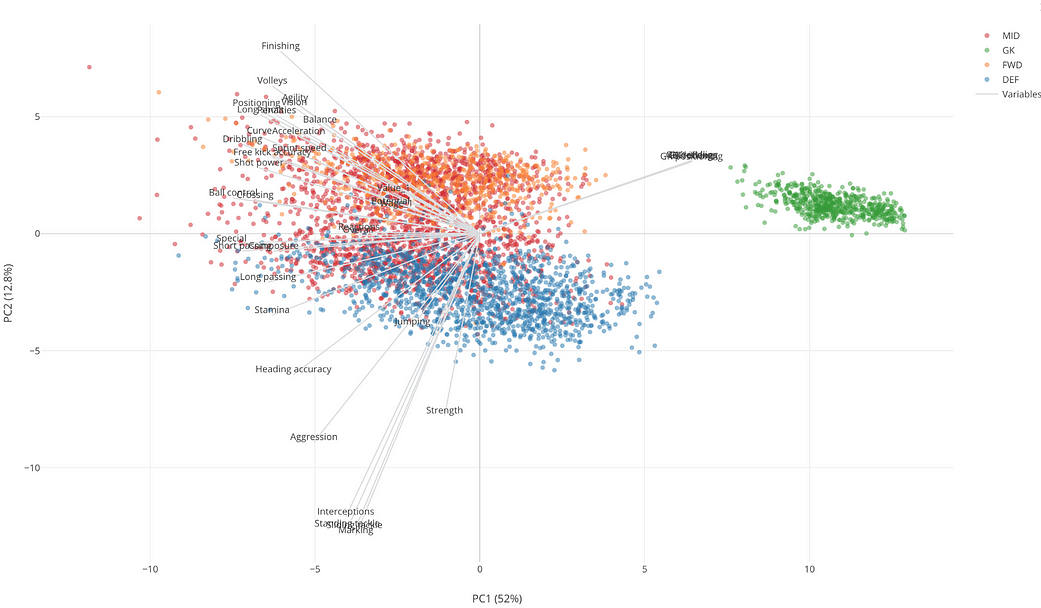
\includegraphics[height=1.70in,width=2.9in,viewport=0 0 1040 620,clip]{Figures/ML_PCM.png}
\caption{\tiny{\textrm{The Schematic diagram of Principal component analysis.}}}%
\label{ML_PCM}
\end{figure}
}

\frame
{
	\frametitle{$k$-\textrm{means}算法}
	$k$-\textrm{means}算法:~{\fontsize{8.0pt}{4.2pt}\selectfont{\textcolor{blue}{直接计算数据点和聚类中心的欧氏距离\textrm{(Euclidean distance)},将$n$个数据分类为$k$个子集($k<n$)}}}
	\vskip 3pt
{\fontsize{8.0pt}{4.2pt}\selectfont{
随机选定聚类中心的个数($k$)和位置($\mathbf{\mu}_0^{(\mathrm{j})}$,$1\leqslant j \leqslant k$),执行迭代:~
\begin{itemize}
	\item 计算每个数据点与聚类中心的距离,标记为$y_t^{\mathrm{(i)}}~(t>0)$,将该点分到距离最小的聚类中心所属的类中
		\begin{displaymath}
			y_t^{(\mathrm{i})}=\textrm{argmin}_j\|\mathbf{x}^{(\mathrm{i})}-\mu_t^{(\mathrm{j})}\|_p
		\end{displaymath}
	\item 重新计算每个聚类的中心$(\{\mu_t^{(\mathrm{j})}\})$
		\begin{displaymath}
			\mu_{t+1}^{(\mathrm{j})}=\dfrac1{n_j}\sum_{i=1}^{n_j}\mathbf{x}^{(\mathrm{i})}\delta_{y_t^{(\mathrm{i})},\mathrm{j}}
		\end{displaymath}
		$p\in\mathbb{N}$表示空间的维度(当$p=2$即为是二维平面的欧氏距离),$n_j$是归入聚类中心$\mu_t^{(\mathrm{j})}$的分类元素数目,$\delta_{n,m}$表示$\Delta$函数,$t$表示迭代次数
\end{itemize}
当标记不再变化时,迭代收敛}}
}

\frame
{
	\frametitle{$k$-\textrm{means}算法}
\begin{figure}[h!]
\centering
\vspace*{-0.1in}
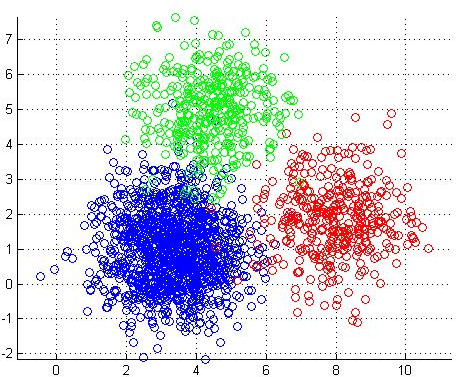
\includegraphics[height=1.80in,width=2.2in,viewport=0 0 110 90,clip]{Figures/ML_k-mean.png}
\caption{\tiny{\textrm{The Schematic diagram of the $k$-means algorithm.}}}%
\label{ML_k-means}
\end{figure}
$k$-\textrm{means}聚类算法的结果与初始聚类中心位置的选择密切关联
\vskip 3pt
{\fontsize{8.0pt}{4.2pt}\selectfont{初始聚类中心选择得不同,结果差别会比较大\footnote{\fontsize{6.0pt}{4.2pt}\selectfont{一般克服的策略是通过多次初始聚类中心并执行该算法,选择最有代表性的聚类形式作为结果}}}}
}

\frame
{
	\frametitle{层次聚类\textrm{(Hierarchical Clustering)}算法}
	层次聚类:~{\fontsize{8.0pt}{4.2pt}\selectfont{\textcolor{blue}{通过一层一层的进行聚类}}}
	\vskip 2pt
	{\fontsize{7.0pt}{4.2pt}\selectfont{\textcolor{magenta}{分裂法}:~由上向下把大的类别分割\\
	\textcolor{magenta}{聚合法}:~由下向上对小的类别聚合}}
{\fontsize{7.0pt}{4.2pt}\selectfont{
\begin{itemize}
	\item 初始时将每个训练数据点$\mathbf{x}^{(\mathrm{i})}$作为一个类(或类簇),原始类大小等于训练数据点数目$n$
	\item 衡量任意两个类(分别标记为\textrm{A}和\textrm{B})的偏差$d(\mathrm{A},\mathrm{B})$
	\item 偏差最小的两个类(最相似)合并一个新的类簇
\end{itemize}
反复执行该聚合过程,最终可以用一个类簇能囊括全部训练集}}
\begin{figure}[h!]
\centering
\vspace*{-0.04in}
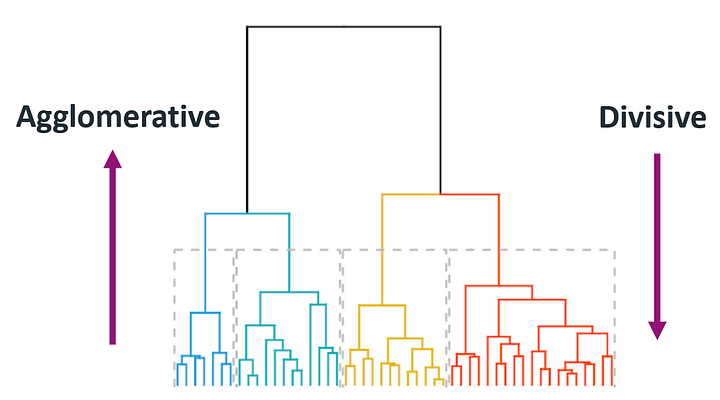
\includegraphics[height=1.47in,width=3.2in,viewport=0 0 730 390,clip]{Figures/ML_Hierarchical-Clustering.png}
\caption{\tiny{\textrm{The Schematic diagram of Hierarchical-Clustering algorithm.}}}%
\label{ML_ML_Hierarchical-Clustering}
\end{figure}
}

\frame
{
	\frametitle{层次聚类\textrm{(Hierarchical Clustering)}算法}
{\fontsize{8.0pt}{4.2pt}\selectfont{
要将$n$个类聚合成$k$个类簇~($1<k<n$)~,要在聚合中对聚合偏差设置截断,常见的聚合截断有三种:
\begin{itemize}
	\item 最小偏差
\begin{displaymath}
	d_{\mathrm{SL}}(\mathrm{A},\mathrm{B})=\min\limits_{i\in\mathrm{A},j\in\mathrm{B}}d_{ij}
\end{displaymath}
$d_{ij}$表示任意一对类的偏差
	\item 最大偏差
\begin{displaymath}
	d_{\mathrm{CL}}(\mathrm{A},\mathrm{B})=\max\limits_{i\in\mathrm{A},j\in\mathrm{B}}d_{ij}
\end{displaymath}
	\item 平均偏差
\begin{displaymath}
	d_{\mathrm{GA}}(\mathrm{A},\mathrm{B})=\dfrac1{|\mathrm{A}||\mathrm{B}|}\sum\limits_{i\in\mathrm{A}}\sum\limits_{j\in\mathrm{B}}d_{ij}
\end{displaymath}
\end{itemize}
定义的$d_{ij}$可以人为指定,对数值形式的数据,最常见的设置为欧氏距离}}
\vskip 5pt
分裂法与聚合法类似,只是初始时训练数据集属于一个类簇,然后逐层分裂形成特定的类簇
}

\frame
{
	\frametitle{线性回归\textrm{(Linear Regression)}算法}
对监督学习来说,每个数据不仅有特征向量$\mathbf{x}_{\mathrm{i}}$,还有相应的值$y_{\mathrm{i}}$
预测连续变化的$y$值,最常用的算法是线性回归
\vskip 3pt
{\fontsize{8.0pt}{4.2pt}\selectfont{回归算法的基本思想:~\textcolor{blue}{对于满足正态分布的数据点}
	\begin{itemize}
			\item 允许的参数拟合预测表达式
\begin{displaymath}
	\hat y^{(\mathrm{i})}=\theta^T\mathbf{x}^{(\mathrm{i})}
\end{displaymath}
{\fontsize{6.0pt}{4.2pt}\selectfont{上标$T$表示矢量的转置,$\hat y^{(\mathrm{i})}$是预测值,$\theta$是参数的矢量}}
		\item 为了求得$\theta$参数,定义误差的最小二乘函数
\begin{displaymath}
	J(\theta)=\sum_{i=1}^nL[\hat{y}^{(\mathrm{i})}(\mathbf{x}^{(\mathrm{i})},\theta),y^{(\mathrm{i})}]=\dfrac12\sum_{i=1}^n(\theta^T\mathbf{x}^{(\mathrm{i})}-y^{(\mathrm{i})})^2
\end{displaymath}
{\fontsize{6.0pt}{4.2pt}\selectfont{最小化该函数,可以得到最优化的参数$\theta$,由此可以得到线性回归机器学习的模型}}
\item 最优化参数$\theta$用矩阵表示可写作:~
\begin{displaymath}
	\theta=(\mathbf{X}^T\mathbf{X})^{-1}\mathbf{X}^T\mathbf{y}
\end{displaymath}
{\fontsize{6.0pt}{4.2pt}\selectfont{这里$\mathbf{X}$矩阵的每一列是由训练集输入数据$\mathbf{x}^{(\mathrm{i})}$,$\mathbf{y}$是对应的输出标注构成的矢量}}
	\end{itemize} }}
}

\frame
{
	\frametitle{预测模型的检验}
机器学习的模型性能,可用测试数据集检验,预测误差与训练数据集包含的数据数量密切相关:
\begin{itemize}
	\item 训练集数据不够,模型不能完全反映训练集特征\\
		{\fontsize{8.0pt}{4.2pt}\selectfont{预测结果将会表现出明显的偏差}}
	\item 训练集数据过多,模型能够体现训练集特征\\
		{\fontsize{8.0pt}{4.2pt}\selectfont{对训练集外的数据效果不好,出现过拟合\textrm{(overfitting)}}}
\end{itemize}
\begin{figure}[h!]
\centering
\vspace*{-0.1in}
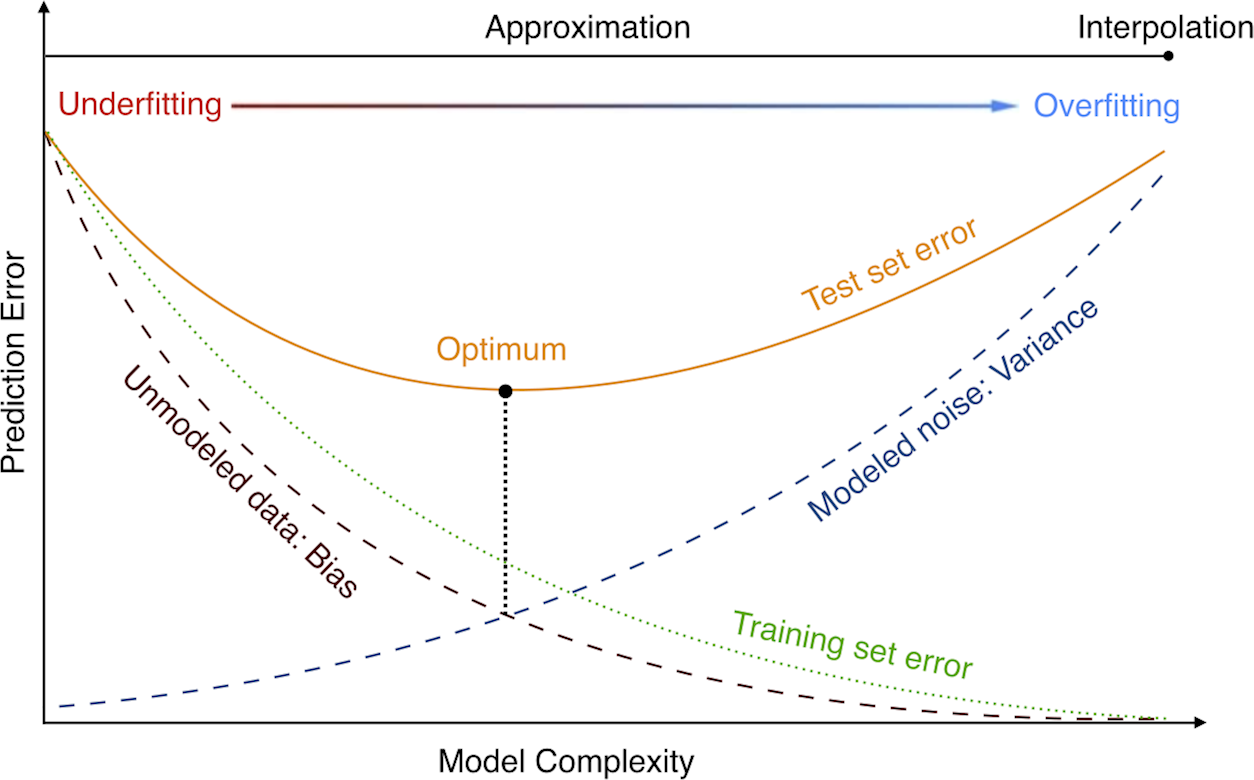
\includegraphics[height=1.4in]{The_optimum_comlexity_vs_prediction.png}
\caption{\tiny{\textrm{Complexity of the model:~Effective number of degrees of freedom (mainly tuned by the hyperparameters of the estimator).}}}%
\label{ML_Fitting_Error}
\end{figure}
}

\frame
{
	\frametitle{预测模型的检验}
回归算法的发展:~构建模型时,通过引入标准化参数$\lambda$来反应训练集元素变化的影响
\begin{displaymath}
	J(\theta)=\dfrac12\sum_{i=1}^n(\theta^T\mathbf{x}^{(\mathrm{i})}-y^{(\mathrm{i})})^2+\lambda\|\theta\|_p
\end{displaymath}
{\fontsize{7.0pt}{4.2pt}\selectfont{这里$p$表示数据度量形式}}
\vskip 4pt
{\fontsize{8.0pt}{4.2pt}\selectfont{优化参数$\lambda$降低训练集数据数量的影响:
	\vskip 3pt
	\textcolor{magenta}{通过压制或筛选训练数据集中的特征来调节其对误差函数的贡献}
\begin{itemize}
	\item $p=1$:~\textrm{Ridge Regression}
	\item $p=2$:~\textrm{LASSO Regression} 
\end{itemize}
\vskip 4pt
注意:~$\lambda$不能像$\theta$一样被优化}}
\vskip 2pt
{\fontsize{6.0pt}{4.2pt}\selectfont{一般是通过比较几个不同的$\lambda$值,选其中能最大化预测能力又不会引入太大偏差的一个}}
}

\frame
{
	\frametitle{分类算法:~逻辑回归\textrm{(logistic regression)}}
}

\frame
{
	\frametitle{深度神经网络基础}
	\begin{itemize}
		\item 感知机(\textrm{Perceptron Learning Algorithm, PLA}):~最早的监督式训练算法,是神经网络构建的基础
\begin{figure}[h!]
\vspace*{-0.08in}
\centering
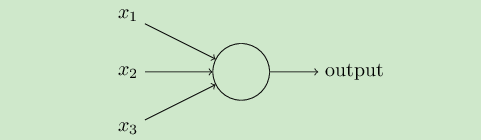
\includegraphics[height=0.50in]{Figures/DNN_PLA.png}
\caption{\tiny \textrm{Perceptron Learning Algorithm.}}%(与文献\cite{EPJB33-47_2003}图1对比)
\label{Fig:PLA}
\end{figure}
输出与输入之间将学习到一个线性关系,可有中间输出结果
\begin{displaymath}
	z=\sum_{i=1}^mw_ix_i+b
\end{displaymath}
中间结果连接一个神经元激活函数
\begin{displaymath}
	\mathrm{sign}(z)=\left\{
		\begin{aligned}
			-1\qquad &z<0\\
			1 \qquad &z\geqslant 0
		\end{aligned}\right.
\end{displaymath}
	\end{itemize}
}

\frame
{
	\frametitle{深度神经网络基础}
\begin{figure}[h!]
\vspace*{-0.08in}
\centering
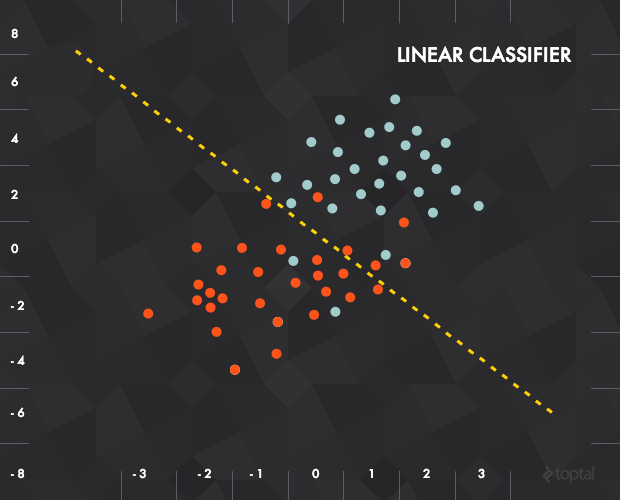
\includegraphics[width=2.5in]{Figures/NN_PLA_example.png}
%\caption{\tiny \textrm{Perceptron Learning Algorithm.}}%(与文献\cite{EPJB33-47_2003}图1对比)
\label{Fig:PLA}
\end{figure}
在本例中,每一个输入数据都可以表示为一个向量$x = (x_1, x_2)$ ,而函数则是要实现“如果线以下,输出0;线以上,输出1”
}

\frame
{
	\frametitle{深度神经网络基础}
感知机模型只能用于二元分类,无法学习较为复杂的非线性模型,神经网络在感知机模型基础上作了扩展
\vskip 10pt
	\begin{itemize}
		\item 加入隐藏层(\textrm{hide layer}):~隐藏层可以有很多层,增强模型的表达能力
		\item 输出层的神经元可以有不止一个输出
		\item 对激活函数作扩展,如\textrm{Sigmoid}函数
			\begin{displaymath}
				f(z)=\dfrac1{1+\mathrm{e}^{-z}}
			\end{displaymath}
			其他的激活函数还有\textrm{tanx}、\textrm{softmax}和\textrm{ReLU}等
	\end{itemize}
}

\frame
{
	\frametitle{深度神经网络}
当前的深度神经网络~\textrm{(Deep Learning Neural Network)}~可以包含上百层神经元,通常有上万个参数,再加上超参数,实际的参数空间几乎是无限大的。如何从海量潜在的可能参数中做选择极具挑战性。
\begin{figure}[h!]
\vspace*{-0.08in}
\centering
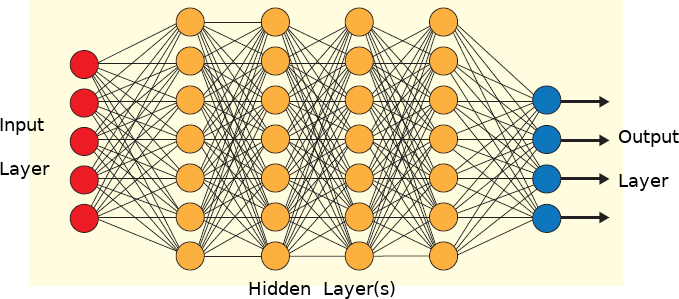
\includegraphics[height=1.75in,width=3.75in]{Figures/ANN_Algorithm.png}
\caption{\tiny \textrm{Deep Learning Neural Network.}}%(与文献\cite{EPJB33-47_2003}图1对比)
\label{Fig:Deep-Learning-NN}
\end{figure}
}

\frame
{
	\frametitle{深度神经网络的前馈算法}
	以三层深度神经网络为例,说明深度神经网络的前馈算法
\begin{figure}[h!]
\vspace*{-0.08in}
\centering
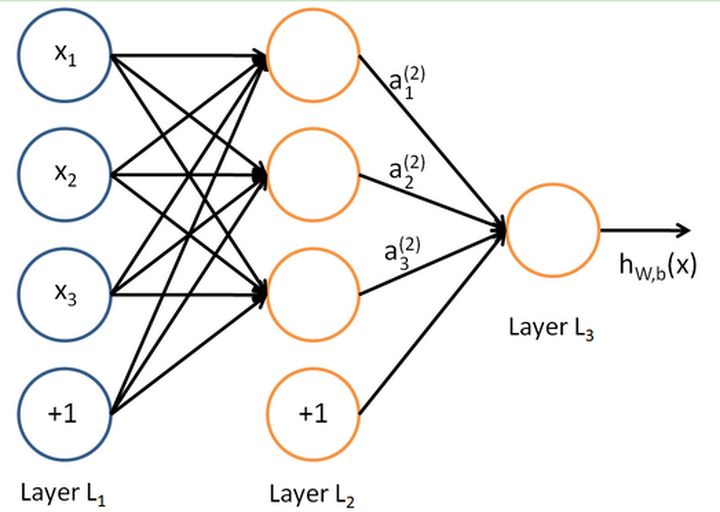
\includegraphics[width=3.0in]{Figures/DNN_front_pro.jpg}
%\caption{\tiny \textrm{Perceptron Learning Algorithm.}}%(与文献\cite{EPJB33-47_2003}图1对比)
\label{Fig:PLA}
\end{figure}
}

\frame
{
	\frametitle{遗传算法的基本原理}
	遗传算法\textrm{(Genetic Algorithm, GA)}是模拟生物进化论的自然选择和遗传学机理的计算模型,\textcolor{blue}{通过模拟自然进化过程搜索最优解}
	\begin{enumerate}
%		\item 优化问题可能潜在的解集构成一个种群(\textrm{population}),该种群由经过基因(\textrm{gene})编码的一定数目的个体(\textrm{individual})组成,每个个体是染色体(\textrm{chromosome})带有特征的实体
		\item 优化问题可能潜在的解集构成一个种群,该种群由经过基因编码的一定数目的个体组成,每个个体是带有一定的优化特征
%		\item 种群产生之后,借助于自然遗传学的遗传算子(\textrm{genetic operators})进行组合交叉(\textrm{crossover})和变异(\textrm{mutation}),产生新一代个体
		\item 种群产生之后,借助于自然遗传学的遗传算子进行组合交叉(\textrm{crossover})和变异(\textrm{mutation}),产生新一代个体
\begin{figure}[h!]
\vspace*{-0.10in}
\centering
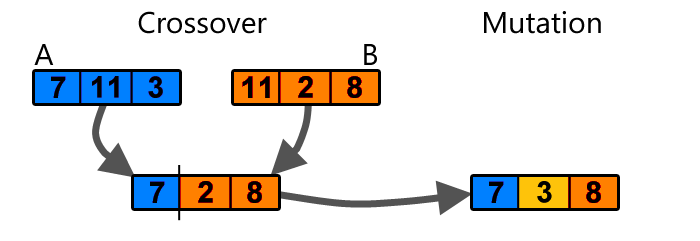
\includegraphics[width=2.5in]{Figures/Genetic_Algorithm_basic.png}
%\caption{\tiny \textrm{Perceptron Learning Algorithm.}}%(与文献\cite{EPJB33-47_2003}图1对比)
\label{Fig:PLA}
\end{figure}
%		\item 按照适者生存和优胜劣汰的原理,在每一代,根据问题域中个体的适应度(\textrm{fitness}),选择(\textrm{selection})合适的个体,构成代表新的解集的种群
\vspace*{-0.10in}
		\item 按照适者生存和优胜劣汰的原理,在每一代,根据问题域中个体的适应度,选择合适的个体,构成代表新的解集的种群
%		\item 逐代(\textrm{generation})演化后,产生出越来越好的近似解(优化目标)
		\item 逐代演化后,产生出越来越好的近似解(优化目标)
	\end{enumerate}
}

\frame
{
	\frametitle{深度神经网络与遗传算法}
	\textcolor{blue}{深度神经网络类似问题的解决方案:~遗传算法}
\begin{minipage}[b]{0.49\textwidth}
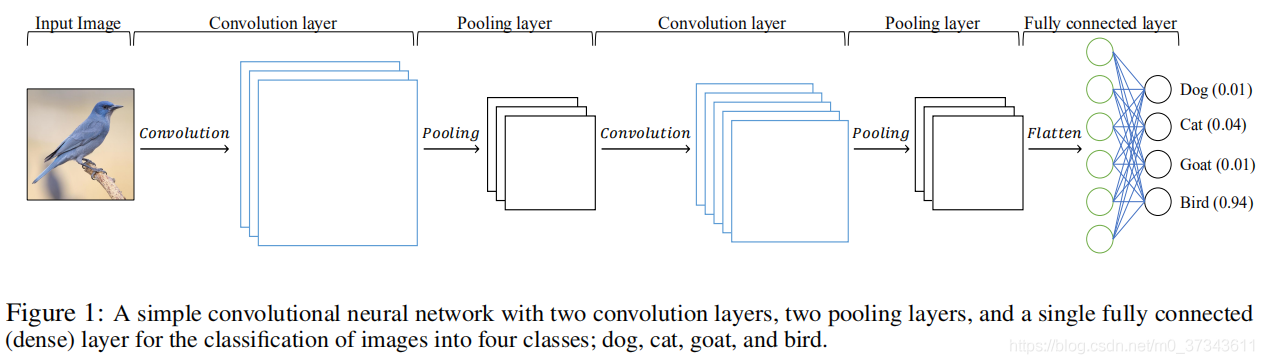
\includegraphics[height=0.4in,width=2.08in,viewport=0 110 1280 350,clip]{Figures/Genetic_Algorithm-2.png}\\
\centering{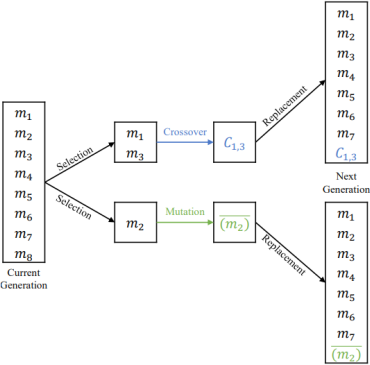
\includegraphics[height=1.0in,width=1.08in,viewport=140 50 820 650,clip]{Figures/Genetic_Algorithm-1.png}}\\
\vskip 0.02pt
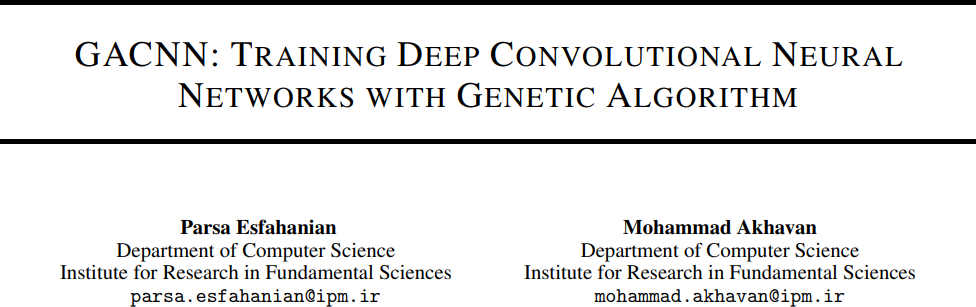
\includegraphics[height=0.7in,width=2.05in]{Figures/Genetic_Algorithm-3.png}\\
\centering{\textcolor{red}{\textrm{\tiny GACNN:~利用遗传算法训练深度卷积神经网络}}}
\end{minipage}
\hfill
\begin{minipage}[b]{0.49\textwidth}
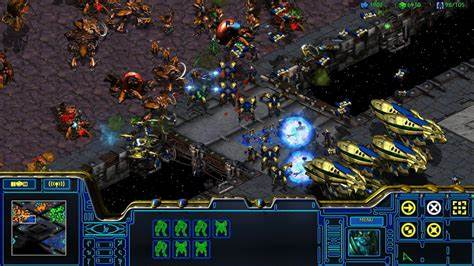
\includegraphics[height=1.2in,width=1.9in]{Figures/Genetic_Algorithm-5.png}\\
\vskip 0.5pt
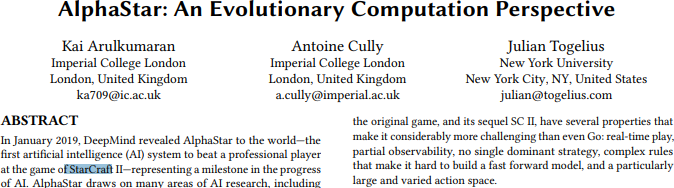
\includegraphics[height=0.55in,width=1.95in]{Figures/Genetic_Algorithm-4.png}\\
\centering{\textcolor{red}{\textrm{\tiny 多智能体强化学习:~神经网络}}}
\end{minipage}
}
